\section{Introduction}
\label{sec:intro}

\textit{Facial emotion recognition} (FER)~\cite{Ko18,JainSS19} is a topic of significant frontier and ongoing debate, 
not only in our daily lives but also in the fields of \textit{artificial intelligence} (AI) and computer vision.
In this report, we aim to leverage several \textit{deep neural networks} (DNNs), 
which contain convolution layers and residual/attention blocks, 
to detect and interpret six basic universally recognized and expressed human facial emotions 
(i.e., happiness, surprise, sadness, anger, disgust, and fear). 
To make our model more transparent, 
we explain this emotion classification task with \textit{class activation mapping} (CAM) 
and \textit{gradient-weighted class activation mapping} (Grad-CAM). 

Our main contributions can be summarized as follows. % update later
\begin{itemize}
  \item We collect and preprocess the training and testing data (image and video) from various public databases. 
  \item We implement all CNN models from scratch and optimize it with different augmentation techniques. 
  Meanwhile, we provide the classification scores of each emotion class in a comprehensive CSV file with respect to each image. 
  \item We give the video demo to illustrate the real-world performance of our best model.
  \item We provide qualitative benefits such as interpretability to explain our model with Grad-CAM. 
\end{itemize}

The structure of this report is arranged as follows. 
\Cref{sec:related} contains the related work of our research. 
In \Cref{sec:approach}, 
we address the datasets we collected and the model architecture we implemented. 
The preliminary evaluation results of our models are given in \Cref{sec:evaluation:results}. 
\Cref{sec:optim} describes the optimization strategies we plan to investigate in the coming weeks. 
\Cref{fig:result} illustrates the empirical results of our current best model. 


% add demo: see https://github.com/werywjw/SEP-CVDL/blob/main/paper/Selvaraju_Cogswell_Grad-CAM.pdf
\section{Related Work}
\label{sec:related}

\subsection{Explainable AI}
\label{sec:related:ai}

\section{Approach}
\label{sec:approach}

\section{Evaluation}
\label{sec:evaluation}

\subsection{Experimental Setup}
\label{sec:evaluation:setup}


\subsection{Dataset Description}
\label{sec:evaluation:datasets}

\begin{table*}[ht]
  \centering
  \begin{tabular}{@{}lccc@{}}
    \toprule
    Dataset & \#Images in training set/Accuracy & \#Images in testing set/Accuracy & \# Images in validation set/Accuracy  \\
    \midrule
    RAF-DB & 9747/98.6 & 2388/83.1 & 600/72.1 \\
    FER+ & 23743/89.6 & 5945/65.6 & 600/40.7  \\
    \bottomrule
  \end{tabular}
  \caption{Overview of the datasets statistics (number of images in respective dataset/accuracy in \%) used in our experiment}
  \label{tab:data}
\end{table*}

To initiate the project, % training, 
we acquired the databases such as FER+~\cite{BarsoumZCZ16}, 
RAF-DB~\cite{li_reliable_2017,li2019reliable}, CK+~\cite{LuceyCKSAM10}, 
TFEID~\cite{tfeid,LiGL22}, 
as well as the video database DISFA~\cite{MavadatiMBTC13}, 
from public institutions and GitHub repositories~\cite{cs229_2023}. 
Based on these databases, we created a dataset by augmentation to increase the variety, 
and full details of augmentation (see \Cref{sec:optim:aug}). 
In terms of illustrating the content of used pictures, we exclusively analyze human faces representing 6 emotions. 
That is, 
we generalized a folder structure annotating the labels 0 (happiness), 1 (surprise), 2 (sadness), 3 (anger), 4 (disgust), and 5 (fear). 
Besides the original format of images and videos, we set standards for extracting frames from the videos, 
resizing training pictures to 64x64 pixels, and saving them in the JPG format.

\begin{figure}[ht]
  \centering
  % \fbox{\rule{0pt}{2in} \rule{0.9\linewidth}{0pt}}
  % \resizebox{.45\textwidth}{!}{
   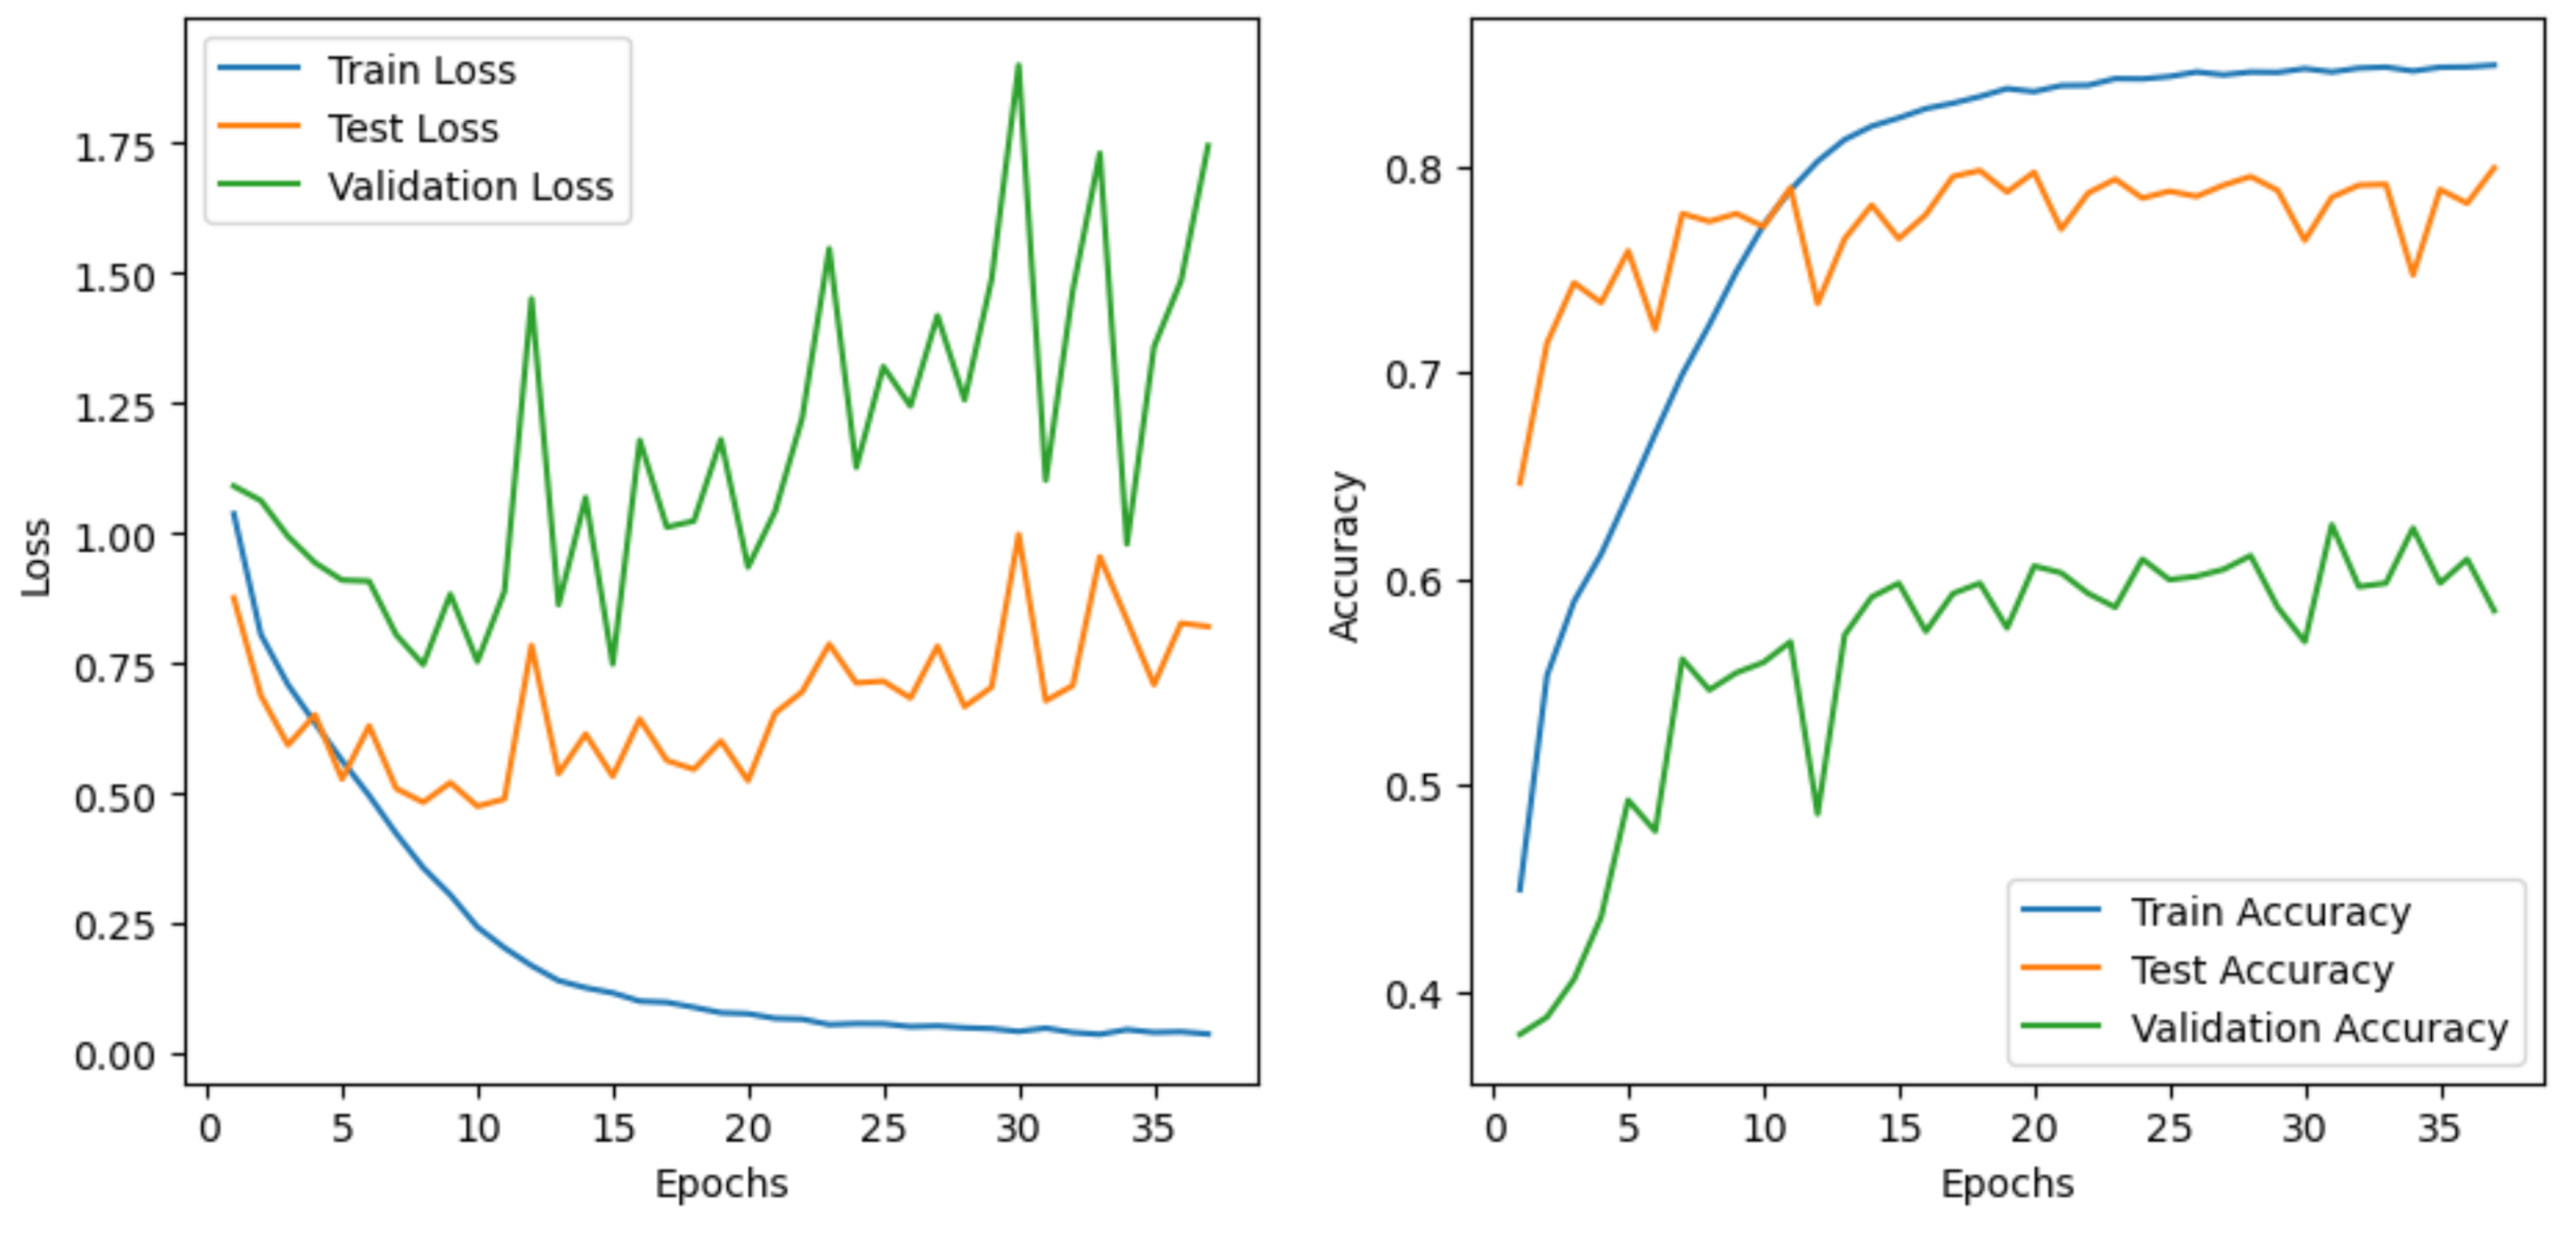
\includegraphics[width=\linewidth]{output.png}
  % }
   \caption{Empirical results in terms of the loss and accuracy with respect to different epochs for our current best model} 
   \label{fig:result}
\end{figure}

The images are converted to greyscale with three channels, 
as our original \textit{convolutional neural network} (CNN) is designed to work with three-channel inputs with random rotation and crop. 
Emotions were assigned tags to each individual picture in a CSV file to facilitate further processing in the model.
We create a custom dataset, which is a collection of data relating to all training images we collected, 
using PyTorch, 
% ~\footnote{\url{https://pytorch.org}}, 
as it includes plenty of existing functions to load various custom datasets in domain libraries such as \texttt{TorchVision}, \texttt{TorchText}, \texttt{TorchAudio}, and \texttt{TorchRec}.

\subsection{Model Architecture}
We implement an emotion classification model from scratch with four convolution layers at the very beginning. 
Following each convolutional layer, 
batch normalization is used, 
as this stabilizes learning by normalizing the input to each layer. 
Afterward, three linear layers are applied to extract features to the final output. 
We also add a dropout layer to prevent overfitting. 
The activation function after each layer is \textit{Rectified Linear Unit} (ReLU), 
since it introduces the non-linearity into the model, 
allowing it to learn more complex patterns. 

In order to find the best hyperparameter configuration (see \Cref{tab:hyper} for details) of the model, 
we utilize the parameter grid from sklearn.
% ~\footnote{\url{https://scikit-learn.org/stable/modules/generated/sklearn.model_selection.ParameterGrid.html}}.
Additionally, we increase the depth of the network by adding some convolutional layers to learn more complex features. 
To help the training of deeper networks more efficiently, 
we add the residual connections, 
as they allow gradients to flow through the network more easily, improving the training for deep architectures. 
Moreover, 
we add \textit{squeeze and excitation} (SE) blocks to apply channel-wise attention. 

\subsection{Results}
\label{sec:evaluation:results}

\begin{table*}[ht]
  \centering
  % \begin{tabular}{l|c|c|c|c|c|c}
  % \begin{tabular}{lcccccc} 
  \begin{tabular}{@{}lcccccc@{}}
  \toprule
  filepath & happiness & surprise & sadness & anger & disgust & fear \\
  \midrule
  archive/RAF-DB/test/test\_0524\_aligned\_happiness.jpg & \textbf{1.00} & 0.00 & 0.00 & 0.00 & 0.00 & 0.00 \\
  archive/RAF-DB/test/test\_0093\_aligned\_happiness.jpg & \textbf{1.00} & 0.00 & 0.00 & 0.00 & 0.00 & 0.00 \\
  archive/RAF-DB/test/test\_2193\_aligned\_sadness.jpg & 0.03 & 0.01 & \textbf{0.90} & 0.01 & 0.02 & 0.04 \\
  archive/RAF-DB/test/test\_1214\_aligned\_happiness.jpg & \textbf{1.00} & 0.00 & 0.00 & 0.00 & 0.00 & 0.00 \\
  archive/RAF-DB/test/test\_1816\_aligned\_surprise.jpg & 0.00 & \textbf{1.00} & 0.00 & 0.00 & 0.00 & 0.00 \\
  archive/RAF-DB/test/test\_0294\_aligned\_surprise.jpg & 0.01 & \textbf{0.99} & 0.00 & 0.00 & 0.00 & 0.00 \\
  archive/RAF-DB/test/test\_1128\_aligned\_happiness.jpg & \textbf{1.00} & 0.00 & 0.00 & 0.00 & 0.00 & 0.00 \\
  archive/RAF-DB/test/test\_1799\_aligned\_sadness.jpg & 0.37 & 0.02 & \textbf{0.45} & 0.02 & 0.1 & 0.03 \\
  archive/RAF-DB/test/test\_0610\_aligned\_sadness.jpg & 0.02 & 0.00 & \textbf{0.74} & 0.02 & 0.21 & 0.01 \\
  archive/RAF-DB/test/test\_1373\_aligned\_anger.jpg & 0.00 & 0.00 & 0.00 & \textbf{1.00} & 0.00 & 0.00 \\
  archive/RAF-DB/test/test\_1788\_aligned\_fear.jpg & 0.00 & 0.00 & 0.00 & 0.00 & 0.00 & \textbf{1.00} \\
  archive/RAF-DB/test/test\_0007\_aligned\_disgust.jpg & 0.03 & 0.05 & 0.03 & \textbf{0.58} & 0.18 & 0.13 \\
  archive/RAF-DB/test/test\_0804\_aligned\_disgust.jpg & 0.02 & 0.00 & 0.18 & 0.02 & \textbf{0.77} & 0.00 \\
  % \vdots & \vdots & \vdots & \vdots & \vdots & \vdots & \vdots \\
  \bottomrule
  \end{tabular}
  \caption{Overview of our random testing results examples extracted from the CSV file}
  \label{tab:testcsv}
\end{table*}  

For evaluation, we use the metric accuracy. 
The loss function employed for all models is cross-entropy, which is typically for multi-class classification. 
We report all the training, testing, and validation accuracy in \% to compare the performance of our models. 

\begin{table}%[ht]
  \centering
  \begin{tabular}{@{}lc@{}}
    \toprule
    Hyperparameter & Value \\
    \midrule
    Learning rate & \{0.1, 0.01, 0.001, 0.0001\}  \\
    Batch size & \{8, 16, 32, 64\} \\
    Dropout rate & \{0.5\} \\
    Epoch & \{30, 40\} \\
    Early stopping & \{\texttt{True}, \texttt{False}\} \\
    Patience & \{5\} \\
    \bottomrule
  \end{tabular}
  \caption{Explored hyperparameter space for our models}
  \label{tab:hyper}
\end{table}

Adding a extra convolutional layer to the model with much more parameters does not necessarily lead to better performance.
Batch normalization can indeed improve the performance of the model. 

% specific dataset comparison, 
% e.g., RAF-DB (train, test, validation) & FER+ (train & test & validation)
% Aggregated train & test (RAF-DB / FER+) & validation 
% bold the best results later

\Cref{fig:result} shows the test result aggregated from the database RAF-DB~\footnote{\url{https://www.kaggle.com/datasets/shuvoalok/raf-db-dataset}}. 
Different combinations of functions from the \texttt{pytorch.transforms} library are tested for augmentation from those already established filters. % that have been developed. 
As seen in \Cref{tab:model}, 
our CNN without random augmentation outperforms the other models in terms of accuracy, 
indicating that this kind of augmentation is not able to help our model predict the correct label, 
thus we later aim to optimize with other augmentation techniques to capture more representative features of different emotions.
Further research is orientated on papers engaging similar investigations~\cite{ZeilerF14,li_reliable_2017,VermaMRMV23}.

\begin{table*}[ht]
  \centering
  % \resizebox{.47\textwidth}{!}{
  \begin{tabular}{@{}lccccc@{}}
    \toprule 
    Models & Architecture &  Accuracy (Train) &  Accuracy (Test) & Accuracy (Vali) & \# params \\
    \midrule
    CNN (6 layers) & +BN-SE & 97.5 & 82.5 & 70.0 & 41950726 \\
    ResNet18~\cite{HeZRS16} & residual block & 98.9 & 81.3 & 67.9 & 11179590 \\
    CNN (5 layers) & -BN-SE & 96.3 & 76.9 & 60.6 & 10474118 \\
    CNN (5 layers) & +BN+SE & 98.4 & 81.7 & 71.1 & 10478598 \\
    CNN (5 layers) & +BN-SE & 98.6 & 83.1 & 72.1 & 10478086 \\
    \bottomrule
  \end{tabular}
  % }
  \caption{Accuracy (\%) for different models in our experiments 
  (Note that Aug stands for data augmentation, SE for squeeze and excitation, and Res for residual connections; 
  +/- represent with/without respectively)}
  \label{tab:model}
\end{table*}

\section{Optimization Strategies}
\label{sec:optim}

% To enhance model performance during training, 
% we will focus on the following tasks, 
% i.e., data augumentation (see \Cref{sec:optim:aug}), 
% CAM (see \Cref{sec:optim:cam}), and Grad-CAM (see \Cref{sec:optim:gcam}). 
%~\footnote{\url{https://github.com/maelfabien/Multimodal-Emotion-Recognition}}. 
% Techniques like dropout, renormalization, and data augmentation are employed 

\subsection{Data Augmentation}
\label{sec:optim:aug}

In deep learning and AI, %machine
augmentation stands as a transformative technique, 
empowering algorithms to learn from and adapt to a wider range of data. 
By introducing subtle modifications to existing data points, 
augmentation effectively expands the dataset, 
enabling models to generalize better and achieve enhanced performance. 
As models encounter slightly altered versions of familiar data, 
they are forced to make more nuanced and robust predictions. 
With this process, we aim to prevent overfitting. % which is a common pitfall in machine learning. 
Additionally, we guide the training process to enhance the recognition and handling of real-world variations.
During the project, we pursue various approaches. 
Meanwhile, we create various replications of existing photos by randomly altering different properties such as size, brightness, color channels, or perspectives.


\subsection{Classification Scores}
\label{sec:optim:csv}
To further analyze the separate scores of each class of the model, 
we write a script that takes a folder path as input and iterates through the images inside a subfolder to record the performance of the model with respect to each emotion class. 
This CSV file is represented with the corresponding classification scores. 

\subsection{CAM and Grad-CAM} % aggregate Class Activation Mapping (CAM)
\label{sec:optim:cam}

In generally, 
CAM~\cite{ZhouKLOT16} helps interpret CNN decisions by providing visual cues about the regions that influenced the classification, 
as it highlights the important regions of an image or a video, 
aiding in the understanding of the behavior of the model, 
which is especially useful for model debugging and improvement. 
Besides proposing a method to visualize the discriminative regions of a CNN trained for the classification task, % classification-trained
we adopt this approach from \citet{ZhouKLOT16} to localize objects without providing the model with any bounding box annotations. 
The model can therefore learn the classification task with class labels and is then able to localize the object of a specific class in an image or video. 

% Technically, CAM generates a heatmap that highlights the important regions of the image in terms of the decision of the model. 
%~\footnote{~\url{https://medium.com/@stepanulyanin/implementing-grad-cam-in-pytorch-ea0937c31e82}}
% CAM is a technique popularly used in CNNs to visualize and understand the regions of an input image that contribute most to a particular class prediction. 
% Model Architecture:
% CAM is typically applied to the final convolutional layer of a CNN, just before the fully connected layers.
% CAM Process:
% The final convolutional layer produces feature maps, and 
% Application: 
% The GAP layer is used to obtain a spatial average of the feature maps. 
% The \textit{global average pooling} (GAP) layer computes the average value of each feature map to obtain a spatial average of feature maps.
% The weights connecting the feature maps to the output class are obtained.
% The weighted combination of feature maps, representing the importance of each spatial location, is used to generate the CAM heatmap.
% CAM is a visualization technique designed to highlight the important regions of an image or video that contribute the most to the prediction of a specific class by a neural network, 
% typically the final convolutional layer of a CNN before the fully connected layers. 
Despite CAM can provide valuable insights into the decision-making process of deep learning models, especially CNNs, 
CAM must be implemented in the last layer of a CNN or before the fully connected layer, 
% Grad-CAM  can be implemented with every architecture without big effort. 
We will meanwhile compare to Gradient-weighted CAM~\cite{SelvarajuCDVPB17}, 
introduced as a technique that is easier to implement with different architectures.
This task will be implemented by using the libraries from PyTorch and OpenCV~\footnote{~\url{https://opencv.org}}.
% \subsection{Grad-CAM} 
% \label{sec:optim:gcam}

\citet{chattopadhay2018grad} proposed Grad-CAM++,

\section{Conclusion and Discussion}
\label{sec:conclusion}

\section{Limitation}
\label{sec:limitation}

\subsection*{Author Contributions}
\label{sec:author}
% see https://arxiv.org/pdf/2005.14165.pdf page42
Equal contributions are listed by alphabetical order of surnames. 
Every author did the literature research and contributed to the writing of the paper. 

\begin{itemize}
  \item \textbf{Tanja Jaschkowitz} implemented the model architecture, training and testing infrastructure, and CSV file aggregations. 
  \item \textbf{Leah Kawka} collected the training data, prepared data processing, implemented augmentation, and ran the results. 
  She also takes part in the explainable AI and Grad-CAM.
  \item \textbf{Mahdi Mohammadi} implemented the augmentation, did the research searching, conclusion reasearching, data preprocessing, and CAM-Images inquiry.
  \item \textbf{Jiawen Wang} implemented the model architecture, training and testing infrastructure, classification score script, and optimization strategies. 
  In the specific writing part, she drew the figures and tables and improved this report from team members.
\end{itemize}

\section*{Acknowledgements}

We are deeply grateful to our advisors \textbf{Johannes Fischer} and \textbf{Ming Gui} for their helpful and valuable support during the entire semester. 
We also thank \textbf{Prof. Dr. Björn Ommer} for providing this interesting practical course.
